%%% Title:    Missing Data in R: Introduction
%%% Author:   Kyle M. Lang
%%% Created:  2015-11-06
%%% Modified: 2022-01-21

\documentclass{beamer}\usepackage[]{graphicx}\usepackage[]{color}
% maxwidth is the original width if it is less than linewidth
% otherwise use linewidth (to make sure the graphics do not exceed the margin)
\makeatletter
\def\maxwidth{ %
  \ifdim\Gin@nat@width>\linewidth
    \linewidth
  \else
    \Gin@nat@width
  \fi
}
\makeatother

\definecolor{fgcolor}{rgb}{0, 0, 0}
\makeatletter
\@ifundefined{AddToHook}{}{\AddToHook{package/xcolor/after}{\definecolor{fgcolor}{rgb}{0, 0, 0}}}
\makeatother
\newcommand{\hlnum}[1]{\textcolor[rgb]{0.69,0.494,0}{#1}}%
\newcommand{\hlstr}[1]{\textcolor[rgb]{0.749,0.012,0.012}{#1}}%
\newcommand{\hlcom}[1]{\textcolor[rgb]{0.514,0.506,0.514}{\textit{#1}}}%
\newcommand{\hlopt}[1]{\textcolor[rgb]{0,0,0}{#1}}%
\newcommand{\hlstd}[1]{\textcolor[rgb]{0,0,0}{#1}}%
\newcommand{\hlkwa}[1]{\textcolor[rgb]{0,0,0}{\textbf{#1}}}%
\newcommand{\hlkwb}[1]{\textcolor[rgb]{0,0.341,0.682}{#1}}%
\newcommand{\hlkwc}[1]{\textcolor[rgb]{0,0,0}{\textbf{#1}}}%
\newcommand{\hlkwd}[1]{\textcolor[rgb]{0.004,0.004,0.506}{#1}}%
\let\hlipl\hlkwb

\usepackage{framed}
\makeatletter
\newenvironment{kframe}{%
 \def\at@end@of@kframe{}%
 \ifinner\ifhmode%
  \def\at@end@of@kframe{\end{minipage}}%
  \begin{minipage}{\columnwidth}%
 \fi\fi%
 \def\FrameCommand##1{\hskip\@totalleftmargin \hskip-\fboxsep
 \colorbox{shadecolor}{##1}\hskip-\fboxsep
     % There is no \\@totalrightmargin, so:
     \hskip-\linewidth \hskip-\@totalleftmargin \hskip\columnwidth}%
 \MakeFramed {\advance\hsize-\width
   \@totalleftmargin\z@ \linewidth\hsize
   \@setminipage}}%
 {\par\unskip\endMakeFramed%
 \at@end@of@kframe}
\makeatother

\definecolor{shadecolor}{rgb}{.97, .97, .97}
\definecolor{messagecolor}{rgb}{0, 0, 0}
\definecolor{warningcolor}{rgb}{1, 0, 1}
\definecolor{errorcolor}{rgb}{1, 0, 0}
\makeatletter
\@ifundefined{AddToHook}{}{\AddToHook{package/xcolor/after}{
\definecolor{shadecolor}{rgb}{.97, .97, .97}
\definecolor{messagecolor}{rgb}{0, 0, 0}
\definecolor{warningcolor}{rgb}{1, 0, 1}
\definecolor{errorcolor}{rgb}{1, 0, 0}
}}
\makeatother
\newenvironment{knitrout}{}{} % an empty environment to be redefined in TeX

\usepackage{alltt}
\usetheme{Utrecht}

\usepackage{graphicx}
\usepackage[natbibapa]{apacite}
\usepackage[libertine]{newtxmath}
\usepackage{fancybox}
\usepackage{booktabs}
\usepackage{eurosym}
\usepackage{caption}

\captionsetup{labelformat = empty}

\title{Missing Data Basics}
\subtitle{Utrecht University Winter School: Missing Data in R}
\author{Kyle M. Lang}
\institute{Department of Methodology \& Statistics\\Utrecht University}
\date{2022-02-03}

%------------------------------------------------------------------------------%

\IfFileExists{upquote.sty}{\usepackage{upquote}}{}
\begin{document}



%------------------------------------------------------------------------------%

\begin{frame}[t, plain]
  \titlepage
\end{frame}

%------------------------------------------------------------------------------%

\begin{frame}{Introduction}

  \begin{enumerate}
  \item What's your name?
    \vc
  \item Where are you from/where do you work?
    \vc
  \item What type of research do you do?
    \vc
  \item What type of missing data problems do you encounter in your research?
    \vc
  \item What statistical software do you use/do you have programming experience?
    \vc
  \item What's your math background?
  \end{enumerate}
  
\end{frame}

%------------------------------------------------------------------------------%

\begin{frame}{Outline}
  \tableofcontents
\end{frame}

%------------------------------------------------------------------------------%

\begin{frame}{A Little Notation}
  
  \begin{align*}
    Y &\coloneqq \text{An $N \times P$ Matrix of Arbitrary Data}\\
    \\
    Y_{mis} &\coloneqq \text{The \emph{missing} part of $Y$}\\
    \\
    Y_{obs} &\coloneqq \text{The \emph{observed} part of $Y$}\\
    \\
    R &\coloneqq \text{An $N \times P$ pattern matrix encoding nonresponse}
  \end{align*}
  
\end{frame}

%------------------------------------------------------------------------------%

\begin{frame}{What are Missing Data?}
  
  Missing data are empty cells in a dataset where there should be observed 
  values.
  \vc
  \begin{itemize}
  \item The missing cells correspond to true population values, but we haven't 
    observed those values.
  \end{itemize}
  \vb 
  \pause
  Not every empty cell is a missing datum.
  \vc
  \begin{itemize}
  \item Quality-of-life ratings for dead patients in a mortality study
    \vc
  \item Firm profitability after the company goes out of business
    \vc
  \item Self-reported severity of menstrual cramping for men
    \vc
  \item Empty blocks of data following ``gateway'' items
  \end{itemize}
  
\end{frame}

%------------------------------------------------------------------------------%
    
\sectionslide{Missing Data Descriptives}

%------------------------------------------------------------------------------%

\begin{frame}{Missing Data Pattern}
  


Missing data (or response) patterns represent unique combinations of observed
and missing items.
\begin{itemize}
  \item $P$ items $\Rightarrow$ $2^P$ possible patterns.
\end{itemize}

\begin{columns}
  \begin{column}{0.45\textwidth}
    
% latex table generated in R 4.1.2 by xtable 1.8-4 package
% Fri Jan 21 14:12:28 2022
\begin{table}[ht]
\centering
\begin{tabular}{ccc}
  \toprule
 & X & Y \\ 
  \midrule
1 & x & y \\ 
  2 & x & . \\ 
  3 & . & y \\ 
  4 & . & . \\ 
   \bottomrule
\end{tabular}
\caption{Patterns for $P = 2$} 
\end{table}

    
  \end{column}
  \begin{column}{0.45\textwidth}
\vx{-12}    
% latex table generated in R 4.1.2 by xtable 1.8-4 package
% Fri Jan 21 14:12:28 2022
\begin{table}[ht]
\centering
\begin{tabular}{cccc}
  \toprule
 & X & Y & Z \\ 
  \midrule
1 & x & y & z \\ 
  2 & x & y & . \\ 
  3 & x & . & z \\ 
  4 & . & y & z \\ 
  5 & x & . & . \\ 
  6 & . & . & z \\ 
  7 & . & y & . \\ 
  8 & . & . & . \\ 
   \bottomrule
\end{tabular}
\caption{Patterns for $P = 3$} 
\end{table}

     
    \end{column}
  \end{columns}
  
\end{frame}

%------------------------------------------------------------------------------%

\begin{frame}{Missing Data Pattern}
  
 The concept of a ``missing data pattern'' can also be used to classify the 
  spatial arrangement of missing cells on a data set.\\
  
  \vc
  
  \begin{itemize}
  \item Univariate
    \begin{itemize}
      \item Missing data occur on only one variable
    \end{itemize}
  
    \vb
  
  \item Monotone
    \begin{itemize}
    \item The proportion of complete elements, in both rows and columns, 
      decreases when traversing the data set.
    \item The observed cells can be arranged into a ``staircase'' pattern.
    \end{itemize}
  
    \vb
  
  \item Arbitrary
    \begin{itemize}
    \item Missing values are ``randomly'' scattered throughout the data set.
    \end{itemize}
  \end{itemize}
  
\end{frame}

\watermarkoff %----------------------------------------------------------------%

\begin{frame}{Example Missing Data Patterns}
  


\begin{columns}[T]
  \begin{column}{0.33\textwidth}
    
% latex table generated in R 4.1.2 by xtable 1.8-4 package
% Fri Jan 21 14:12:28 2022
\begin{table}[ht]
\centering
\begin{tabular}{cccc}
  \toprule
 & X & Y & Z \\ 
  \midrule
1 & x & y & z \\ 
  2 & x & y & z \\ 
  3 & x & y & z \\ 
  4 & x & y & z \\ 
  5 & x & y & z \\ 
  6 & x & . & z \\ 
  7 & x & . & z \\ 
  8 & x & . & z \\ 
  9 & x & . & z \\ 
  10 & x & . & z \\ 
   \bottomrule
\end{tabular}
\caption{Univariate Pattern} 
\end{table}


\end{column}
\begin{column}{0.33\textwidth}
  
% latex table generated in R 4.1.2 by xtable 1.8-4 package
% Fri Jan 21 14:12:28 2022
\begin{table}[ht]
\centering
\begin{tabular}{cccc}
  \toprule
 & X & Y & Z \\ 
  \midrule
1 & x & y & z \\ 
  2 & x & y & z \\ 
  3 & x & y & z \\ 
  4 & x & y & . \\ 
  5 & x & y & . \\ 
  6 & x & y & . \\ 
  7 & x & . & . \\ 
  8 & x & . & . \\ 
  9 & x & . & . \\ 
  10 & . & . & . \\ 
   \bottomrule
\end{tabular}
\caption{Monotone Pattern} 
\end{table}

  
\end{column}
\begin{column}{0.33\textwidth}
  
% latex table generated in R 4.1.2 by xtable 1.8-4 package
% Fri Jan 21 14:12:28 2022
\begin{table}[ht]
\centering
\begin{tabular}{cccc}
  \toprule
 & X & Y & Z \\ 
  \midrule
1 & x & . & z \\ 
  2 & x & y & z \\ 
  3 & x & y & z \\ 
  4 & x & . & z \\ 
  5 & x & y & z \\ 
  6 & x & . & z \\ 
  7 & . & y & z \\ 
  8 & x & y & z \\ 
  9 & x & . & . \\ 
  10 & x & y & . \\ 
   \bottomrule
\end{tabular}
\caption{Arbitrary Pattern} 
\end{table}

  
\end{column}
\end{columns}

\end{frame}

\watermarkon %-----------------------------------------------------------------%

\begin{frame}[allowframebreaks]{Nonresponse Rates}
  
  \textsc{Percent/Proportion Missing}
  \begin{itemize}
  \item The proportion of cells containing missing data
  \item Good early screening measure
  \item Should be computed for each variable, not for the entire dataset
  \end{itemize}
  
  \va
  
  \textsc{Attrition Rate}
  \begin{itemize}
  \item The proportion of participants that drop-out of a study at each 
    measurement occasion
  \end{itemize}
  
  \va
  
  \textsc{Percent/Proportion of Complete Cases}
  \begin{itemize}
  \item The proportion of observations with no missing data
  \item Often reported but nearly useless quantity
  \end{itemize}
  
  \pagebreak
  
  \textsc{Covariance Coverage}
  \begin{itemize}
  \item The proportion of cases available to estimate a given pairwise
    relationship (e.g., a covariance between two variables)
  \item Very important to have adequate coverage of the parameters you
    want to estimate
  \end{itemize}
  
  \va
  
  \textsc{Fraction of Missing Information}
  \begin{itemize}
  \item Associated with an estimated parameter, not with an incomplete variable
  \item Like an $R^2$ for the missing data
  \item Most important diagnostic value for missing data problems
  \item Can only be computed after treating the missing data
  \end{itemize}
  
  \pagebreak
  
  \textsc{Influx}
  \begin{itemize}
  \item Foo
  \end{itemize}
  
  \va
  
  \textsc{Outflux}
  \begin{itemize}
  \item Bar
  \end{itemize}
  
\end{frame}

\watermarkoff %----------------------------------------------------------------%

\begin{frame}{Covariance Coverage Examples}
  
  \begin{columns}
    \begin{column}{0.5\textwidth}
      
      \begin{itemize}
      \item What is the coverage for $cov(X, Y)$?
        \vc
      \item What is the coverage for $cov(W, Y)$?
        \vc
      \item What about $cov(X, Z)$?
      \end{itemize}
      
    \end{column}
    \begin{column}{0.5\textwidth}
      
% latex table generated in R 4.1.2 by xtable 1.8-4 package
% Fri Jan 21 14:12:28 2022
\begin{table}[ht]
\centering
\begin{tabular}{ccccc}
  \toprule
 & W & X & Y & Z \\ 
  \midrule
1 & w & x & y & . \\ 
  2 & w & x & y & . \\ 
  3 & w & x & y & . \\ 
  4 & w & x & y & . \\ 
  5 & w & x & y & . \\ 
  6 & w & . & y & z \\ 
  7 & w & . & y & z \\ 
  8 & w & . & y & z \\ 
  9 & w & . & y & z \\ 
  10 & w & . & y & z \\ 
   \bottomrule
\end{tabular}
\end{table}


\end{column}
\end{columns}
 
\end{frame}

%------------------------------------------------------------------------------%

\begin{frame}{Nonresponse Rate Examples}
  
  \begin{columns}
    \begin{column}{0.5\textwidth}
      
      \begin{itemize}
        \item What is the percent missing at Time 2?
          \vc
        \item What is the attrition rate at Time 3?
      \end{itemize}
      
    \end{column}
    \begin{column}{0.5\textwidth}
      
% latex table generated in R 4.1.2 by xtable 1.8-4 package
% Fri Jan 21 14:12:28 2022
\begin{table}[ht]
\centering
\begin{tabular}{ccccc}
  \toprule
 & T1 & T2 & T3 & T4 \\ 
  \midrule
1 & x1 & x2 & x3 & x4 \\ 
  2 & x1 & x2 & x3 & x4 \\ 
  3 & x1 & x2 & x3 & x4 \\ 
  4 & x1 & x2 & x3 & . \\ 
  5 & x1 & x2 & x3 & . \\ 
  6 & x1 & x2 & . & . \\ 
  7 & x1 & x2 & . & . \\ 
  8 & x1 & . & . & . \\ 
  9 & x1 & . & . & . \\ 
  10 & x1 & . & . & . \\ 
   \bottomrule
\end{tabular}
\end{table}


\end{column}
\end{columns}

\end{frame}

\watermarkon %-----------------------------------------------------------------%

\sectionslide{Missing Data Mechanisms}

%------------------------------------------------------------------------------%

\begin{frame}{Missing Data Mechanisms}

  MCAR:
  \begin{align*}
    P(R | Y_{mis}, Y_{obs}) = P(R)
  \end{align*}
  MAR:
  \begin{align*}
    P(R | Y_{mis}, Y_{obs}) = P(R | Y_{obs})
  \end{align*}
  MNAR:
  \begin{align*}
    P(R | Y_{mis}, Y_{obs}) \neq P(R | Y_{obs})
  \end{align*}
  
\end{frame}

\watermarkoff %----------------------------------------------------------------%

\begin{frame}[fragile]{Simulate Some Toy Data}
  
\begin{knitrout}\footnotesize
\definecolor{shadecolor}{rgb}{0.878, 0.918, 0.933}\color{fgcolor}\begin{kframe}
\begin{alltt}
\hlstd{nObs} \hlkwb{<-} \hlnum{5000} \hlcom{# Sample Size}
\hlstd{pm}   \hlkwb{<-} \hlnum{0.3}  \hlcom{# Proportion Missing}

\hlstd{sigma} \hlkwb{<-} \hlkwd{matrix}\hlstd{(}\hlkwd{c}\hlstd{(}\hlnum{1.0}\hlstd{,} \hlnum{0.5}\hlstd{,} \hlnum{0.0}\hlstd{,}
                  \hlnum{0.5}\hlstd{,} \hlnum{1.0}\hlstd{,} \hlnum{0.3}\hlstd{,}
                  \hlnum{0.0}\hlstd{,} \hlnum{0.3}\hlstd{,} \hlnum{1.0}\hlstd{),}
                \hlkwc{ncol} \hlstd{=} \hlnum{3}\hlstd{)}
\hlstd{simDat} \hlkwb{<-} \hlkwd{as.data.frame}\hlstd{(}\hlkwd{rmvnorm}\hlstd{(nObs,} \hlkwd{c}\hlstd{(}\hlnum{0}\hlstd{,} \hlnum{0}\hlstd{,} \hlnum{0}\hlstd{), sigma))}
\hlkwd{colnames}\hlstd{(simDat)} \hlkwb{<-} \hlkwd{c}\hlstd{(}\hlstr{"y"}\hlstd{,} \hlstr{"x"}\hlstd{,} \hlstr{"z"}\hlstd{)}

\hlstd{x} \hlkwb{<-} \hlstd{simDat}\hlopt{$}\hlstd{x}
\hlstd{y} \hlkwb{<-} \hlstd{simDat}\hlopt{$}\hlstd{y}
\hlstd{z} \hlkwb{<-} \hlstd{simDat}\hlopt{$}\hlstd{z}

\hlkwd{cor}\hlstd{(y, x)} \hlcom{# Check correlation between X and Y}
\end{alltt}
\begin{verbatim}
[1] 0.5031885
\end{verbatim}
\end{kframe}
\end{knitrout}

\end{frame}

%------------------------------------------------------------------------------%

\begin{frame}[fragile, allowframebreaks]{MCAR Example}
  
\begin{knitrout}\footnotesize
\definecolor{shadecolor}{rgb}{0.878, 0.918, 0.933}\color{fgcolor}\begin{kframe}
\begin{alltt}
\hlcom{## Simulate MCAR Missingness:}
\hlstd{rVec1} \hlkwb{<-} \hlkwd{sample}\hlstd{(}\hlnum{1} \hlopt{:} \hlkwd{length}\hlstd{(y),} \hlkwc{size} \hlstd{= pm} \hlopt{*} \hlkwd{length}\hlstd{(y))}

\hlstd{y2} \hlkwb{<-} \hlstd{y}
\hlstd{y2[rVec1]} \hlkwb{<-} \hlnum{NA}

\hlkwd{cor}\hlstd{(y2, x,} \hlkwc{use} \hlstd{=} \hlstr{"pairwise"}\hlstd{)} \hlcom{# Look at correlation}
\end{alltt}
\begin{verbatim}
[1] 0.5229792
\end{verbatim}
\end{kframe}
\end{knitrout}

\pagebreak

\begin{knitrout}\footnotesize
\definecolor{shadecolor}{rgb}{0.878, 0.918, 0.933}\color{fgcolor}

{\centering 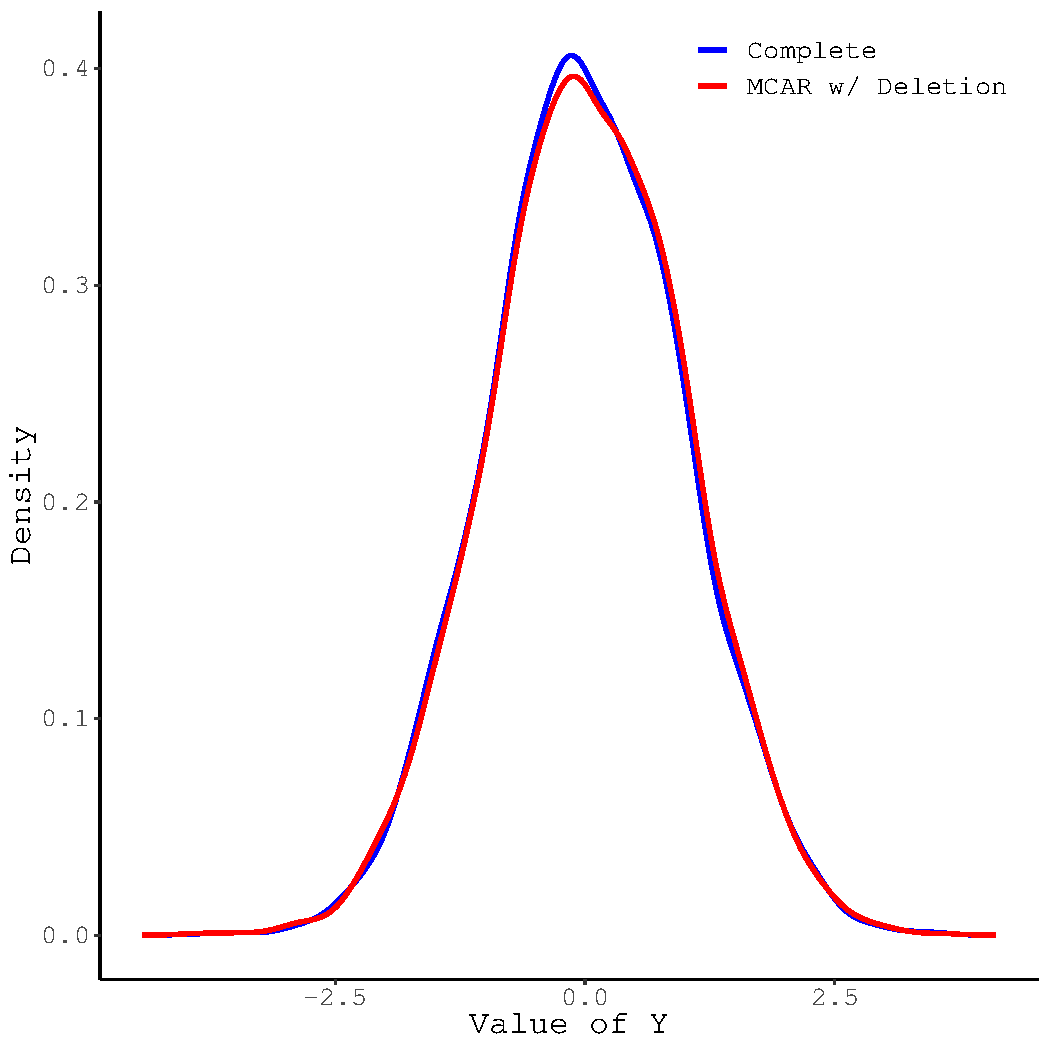
\includegraphics[width=0.65\linewidth]{figure/intro-unnamed-chunk-12-1} 

}


\end{knitrout}

\end{frame}

%------------------------------------------------------------------------------%

\begin{frame}[fragile, allowframebreaks]{MAR Example}
  
\begin{knitrout}\footnotesize
\definecolor{shadecolor}{rgb}{0.878, 0.918, 0.933}\color{fgcolor}\begin{kframe}
\begin{alltt}
\hlcom{## Simulate MAR Missingness:}
\hlstd{rVec2} \hlkwb{<-} \hlstd{x} \hlopt{<} \hlkwd{quantile}\hlstd{(x,} \hlkwc{probs} \hlstd{= pm)}
\hlkwd{mean}\hlstd{(rVec2)}
\end{alltt}
\begin{verbatim}
[1] 0.3
\end{verbatim}
\begin{alltt}
\hlstd{y3} \hlkwb{<-} \hlstd{y}
\hlstd{y3[rVec2]} \hlkwb{<-} \hlnum{NA}

\hlkwd{cor}\hlstd{(y3, x,} \hlkwc{use} \hlstd{=} \hlstr{"pairwise"}\hlstd{)} \hlcom{# Not looking so good :(}
\end{alltt}
\begin{verbatim}
[1] 0.3870092
\end{verbatim}
\end{kframe}
\end{knitrout}

\pagebreak

\begin{knitrout}\footnotesize
\definecolor{shadecolor}{rgb}{0.878, 0.918, 0.933}\color{fgcolor}

{\centering 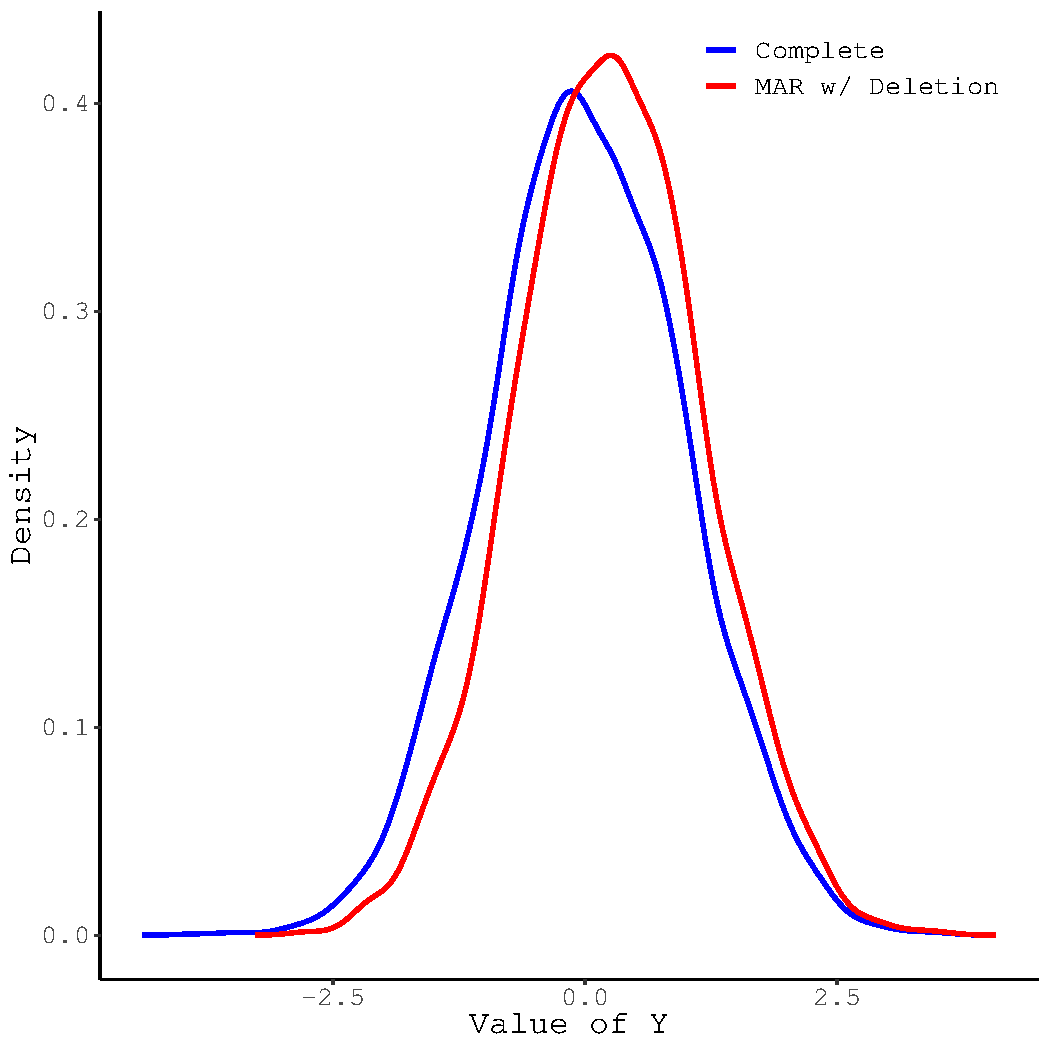
\includegraphics[width=0.65\linewidth]{figure/intro-unnamed-chunk-14-1} 

}


\end{knitrout}

\end{frame}

%------------------------------------------------------------------------------%

\begin{frame}[fragile, allowframebreaks]{MNAR Example}
  
\begin{knitrout}\footnotesize
\definecolor{shadecolor}{rgb}{0.878, 0.918, 0.933}\color{fgcolor}\begin{kframe}
\begin{alltt}
\hlcom{## Simulate MNAR Missingness:}
\hlstd{rVec3} \hlkwb{<-} \hlstd{y} \hlopt{<} \hlkwd{quantile}\hlstd{(y,} \hlkwc{probs} \hlstd{= pm)}
\hlkwd{mean}\hlstd{(rVec3)}
\end{alltt}
\begin{verbatim}
[1] 0.3
\end{verbatim}
\begin{alltt}
\hlstd{y4} \hlkwb{<-} \hlstd{y}
\hlstd{y4[rVec3]} \hlkwb{<-} \hlnum{NA}

\hlkwd{cor}\hlstd{(y4, x,} \hlkwc{use} \hlstd{=} \hlstr{"pairwise"}\hlstd{)} \hlcom{# Hmm...looks pretty bad.}
\end{alltt}
\begin{verbatim}
[1] 0.3873756
\end{verbatim}
\end{kframe}
\end{knitrout}

\pagebreak

\begin{knitrout}\footnotesize
\definecolor{shadecolor}{rgb}{0.878, 0.918, 0.933}\color{fgcolor}

{\centering 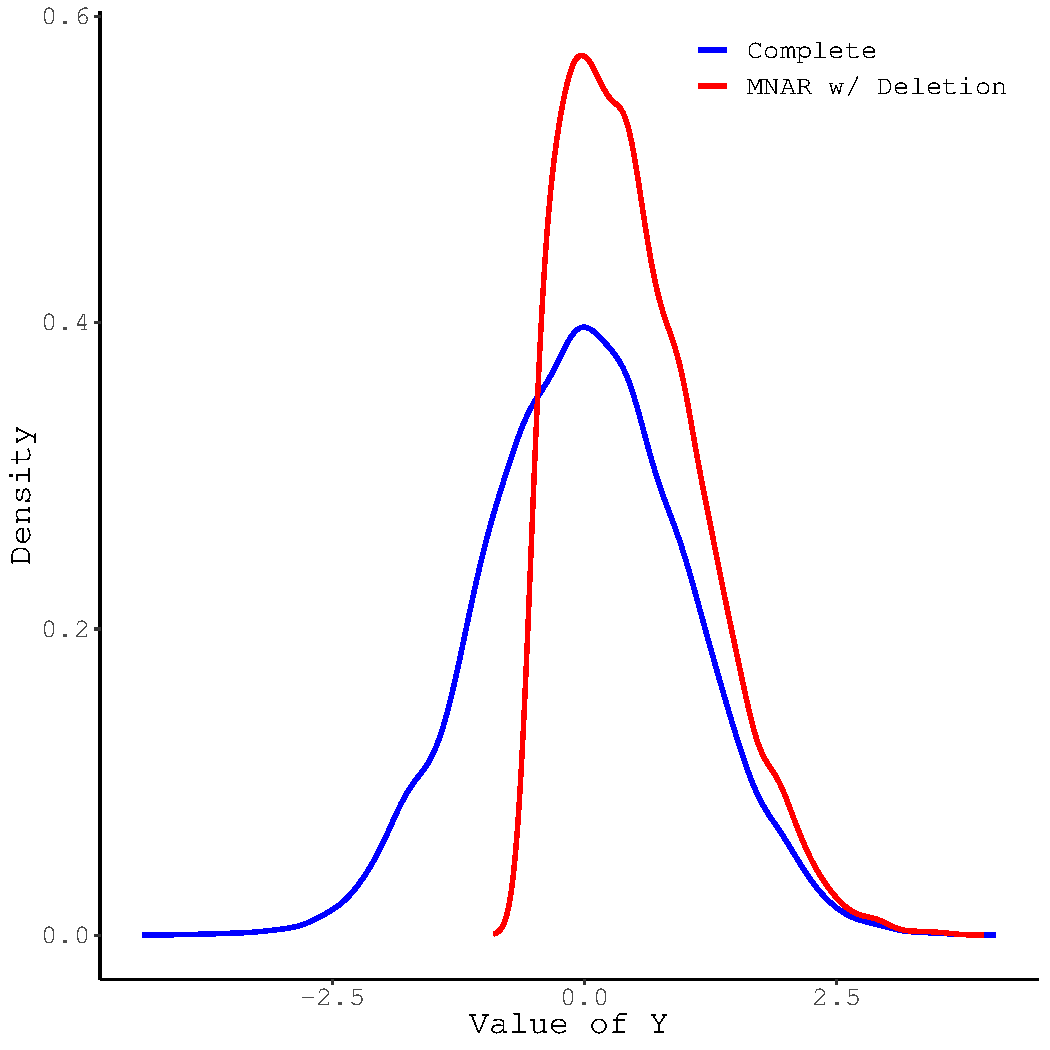
\includegraphics[width=0.65\linewidth]{figure/intro-unnamed-chunk-16-1} 

}


\end{knitrout}

\end{frame}

%------------------------------------------------------------------------------%

\begin{frame}[fragile]{Crucial Nuance}
  
  In our previous MAR example, ignoring the predictor of missingness actually 
  produces \emph{Indirect MNAR}.\\
  
  \pause
  \va
  
  \textsc{Question:} What happens if we ignore the predictor of missingness, but
  that predictor is independent of our study variables?
  
  \pause
  
\begin{knitrout}\footnotesize
\definecolor{shadecolor}{rgb}{0.878, 0.918, 0.933}\color{fgcolor}\begin{kframe}
\begin{alltt}
\hlstd{rVec3}     \hlkwb{<-} \hlstd{z} \hlopt{<} \hlkwd{quantile}\hlstd{(z,} \hlkwc{probs} \hlstd{= pm)}
\hlstd{y5}        \hlkwb{<-} \hlstd{y}
\hlstd{y5[rVec3]} \hlkwb{<-} \hlnum{NA}

\hlkwd{cor}\hlstd{(y5, x,} \hlkwc{use} \hlstd{=} \hlstr{"pairwise"}\hlstd{)}
\end{alltt}
\begin{verbatim}
[1] 0.5161666
\end{verbatim}
\end{kframe}
\end{knitrout}

\textsc{Answer:} We get back to MCAR :)

\end{frame}

%------------------------------------------------------------------------------%

\begin{frame}{Crucial Nuance}
  
  The missing data mechanisms are not simply characteristics of an incomplete 
  dataset; we also need to account for the analysis.
  \vb
  \begin{columns}
    \begin{column}{0.5\textwidth}
      
\begin{knitrout}\footnotesize
\definecolor{shadecolor}{rgb}{0.878, 0.918, 0.933}\color{fgcolor}

{\centering 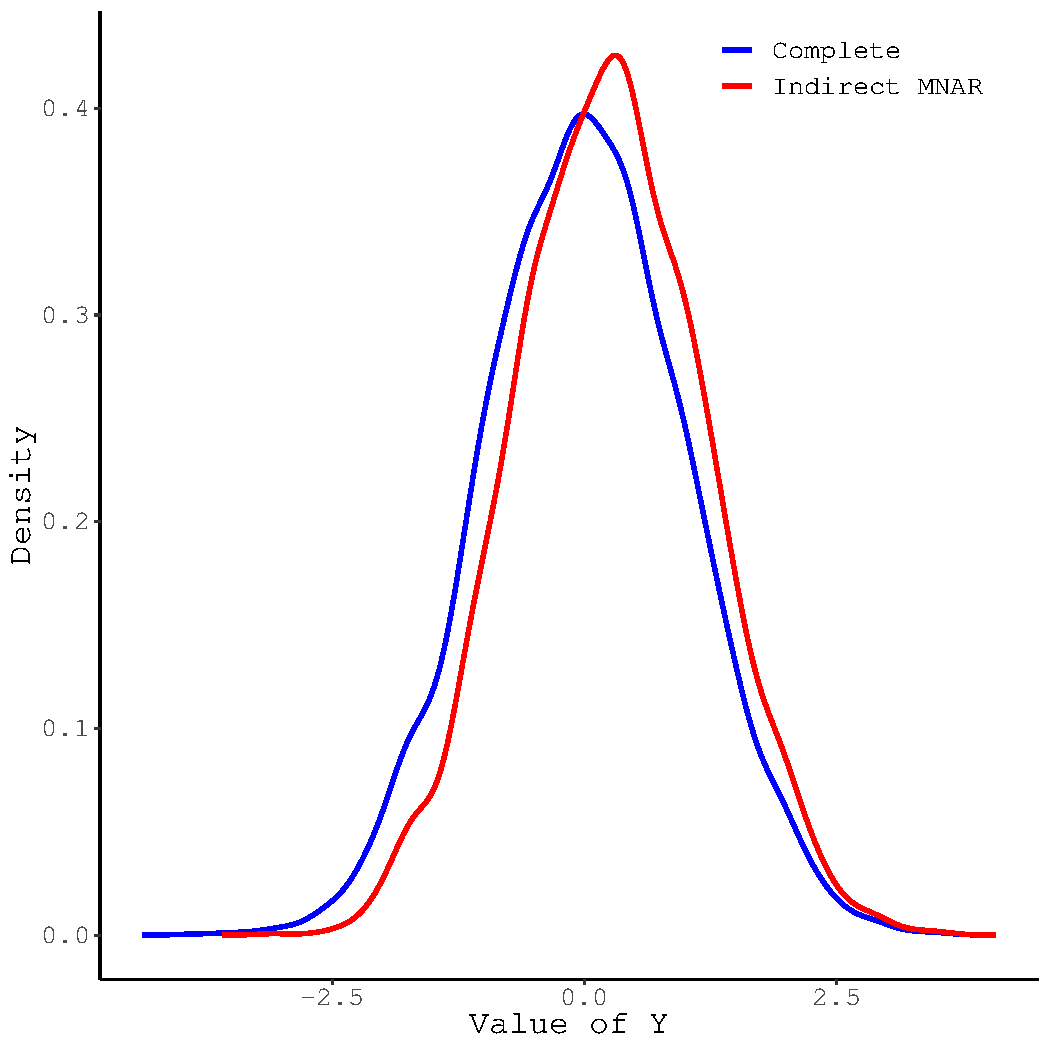
\includegraphics[width=1\linewidth]{figure/intro-unnamed-chunk-18-1} 

}


\end{knitrout}

\end{column}
\begin{column}{0.5\textwidth}
  
\begin{knitrout}\footnotesize
\definecolor{shadecolor}{rgb}{0.878, 0.918, 0.933}\color{fgcolor}

{\centering 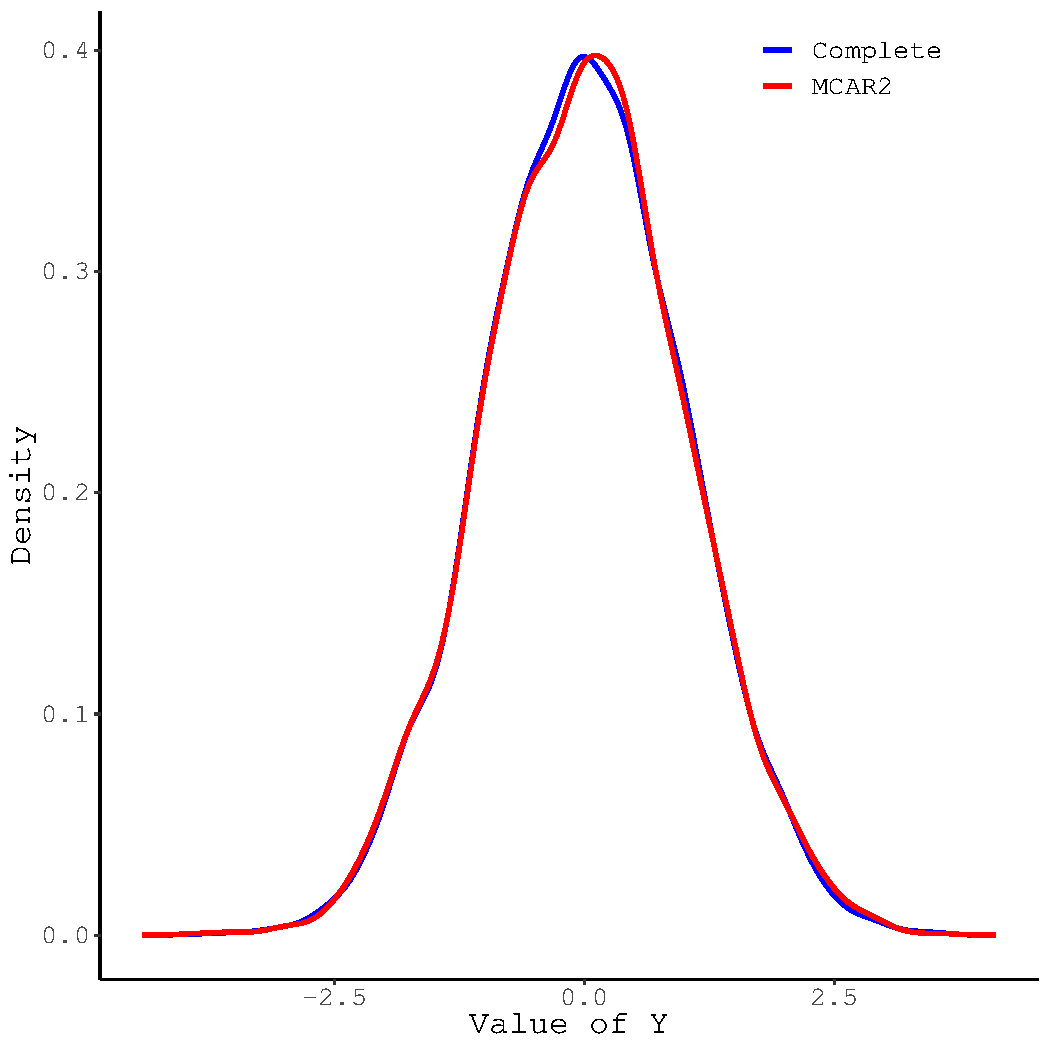
\includegraphics[width=1\linewidth]{figure/intro-unnamed-chunk-19-1} 

}


\end{knitrout}
  
\end{column}
\end{columns}

\end{frame}

\watermarkon %-----------------------------------------------------------------%

\begin{frame}{Testing the Missing Data Mechanism}
  
  We cannot test for MAR or MNAR.
  \begin{itemize}
  \item To do so would require knowing the values of the missing data.
  \end{itemize}
  \vb
  We can test for MCAR (sort of).
  \begin{itemize}
  \item With MCAR, the missing data and the observed data should have the same distribution.
  \item We can test for MCAR by testing the distributions of \emph{auxiliary variables}, $Z$.
    \begin{itemize}
      \item Use a $t$-test to compare the subset of $Z$ that corresponds to 
        $Y_{mis}$ to the subset corresponding to $Y_{obs}$.
    \end{itemize}
  \end{itemize}
  
\end{frame}

%------------------------------------------------------------------------------%

\begin{frame}{Little's MCAR Test}
  
\end{frame}

%------------------------------------------------------------------------------%

\sectionslide{Missing Data Treatments}

%------------------------------------------------------------------------------%

\begin{frame}{Bad Methods (These almost never work)}
   
  Listwise Deletion (Complete Case Analysis)
  \begin{itemize}
  \item Use only complete observations for the analysis
    \begin{itemize}
    \item Very wasteful (can throw out lots of useful data)
    \item Loss of statistical power
    \end{itemize}
  \end{itemize}

  \va
  
  Pairwise Deletion (Available Case Analysis)
  \begin{itemize}
  \item Use only complete pairs of observations for analysis
    \begin{itemize}
    \item Different samples sizes for different parameter estimates
    \item Can cause computational issues 
    \end{itemize}
  \end{itemize}
  
\end{frame}

\watermarkoff %----------------------------------------------------------------%

\begin{frame}{Bad Methods (These almost never work)}
  
  \begin{columns}
    \begin{column}{0.5\textwidth}
      
      (Unconditional) Mean Substitution
      \begin{itemize}
      \item Replace $Y_{mis}$ with $\bar{Y}_{obs}$
        \begin{itemize}
        \item Negatively biases regression slopes and correlations
        \item Attenuates measures of linear association
        \end{itemize}
      \end{itemize}
      
    \end{column}
    \begin{column}{0.5\textwidth}
      
\begin{knitrout}\footnotesize
\definecolor{shadecolor}{rgb}{0.878, 0.918, 0.933}\color{fgcolor}

{\centering 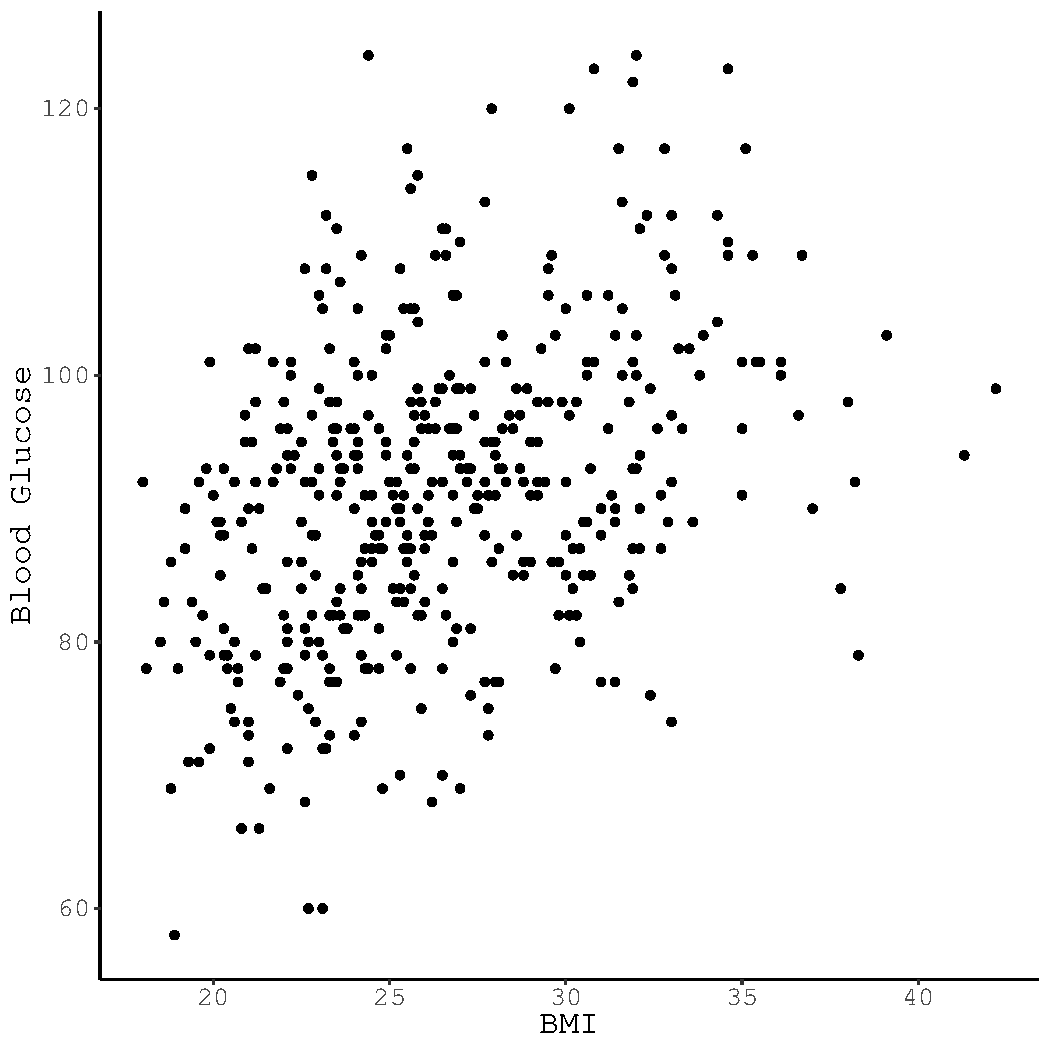
\includegraphics[width=\maxwidth]{figure/intro-unnamed-chunk-20-1} 

}


\end{knitrout}

\end{column}
\end{columns}

\end{frame}

%------------------------------------------------------------------------------%

\begin{frame}{Bad Methods (These almost never work)}
  
  \begin{columns}
    \begin{column}{0.5\textwidth}
      
      (Unconditional) Mean Substitution
      \begin{itemize}
      \item Replace $Y_{mis}$ with $\bar{Y}_{obs}$
        \begin{itemize}
        \item Negatively biases regression slopes and correlations
        \item Attenuates measures of linear association
        \end{itemize}
      \end{itemize}
      
    \end{column}
    \begin{column}{0.5\textwidth}
      
\begin{knitrout}\footnotesize
\definecolor{shadecolor}{rgb}{0.878, 0.918, 0.933}\color{fgcolor}

{\centering 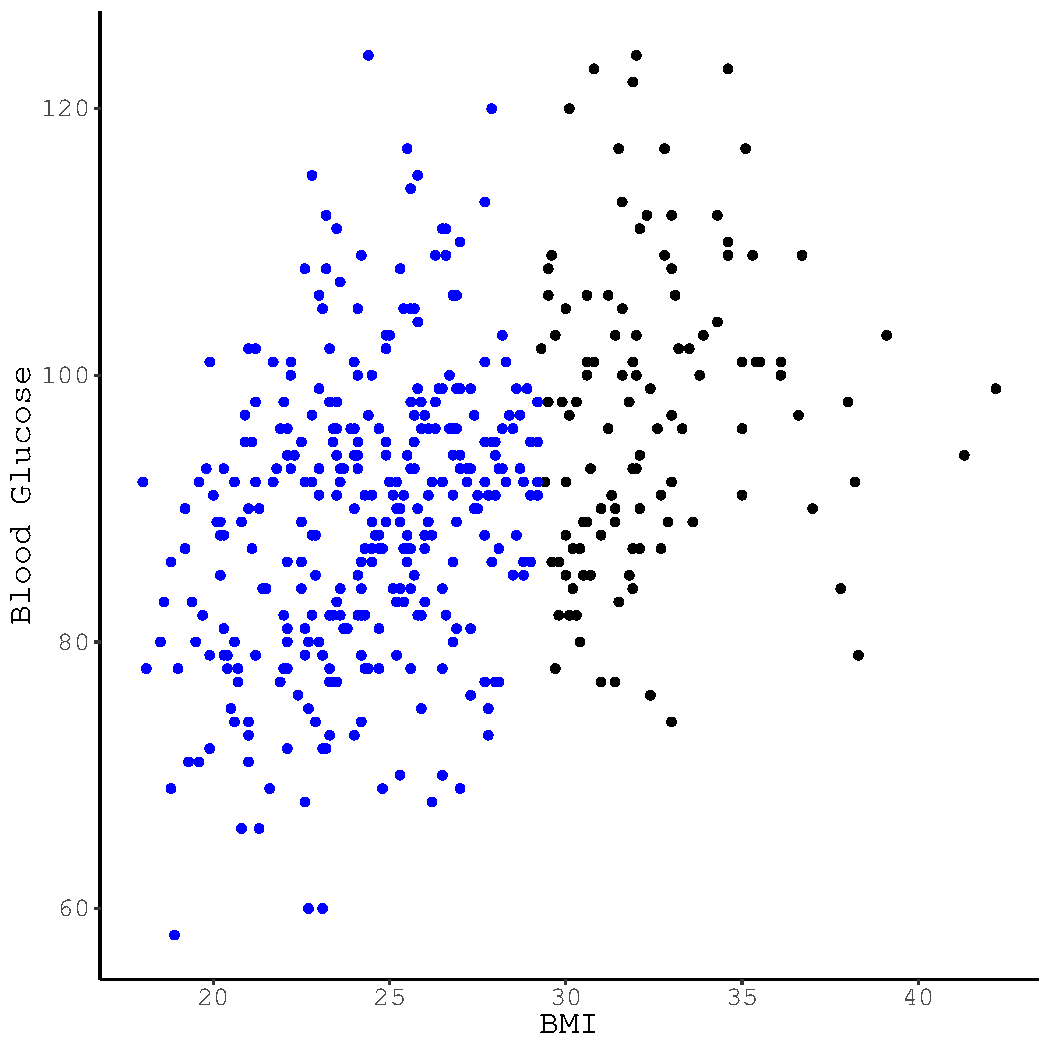
\includegraphics[width=\maxwidth]{figure/intro-unnamed-chunk-21-1} 

}


\end{knitrout}

\end{column}
\end{columns}

\end{frame}

%------------------------------------------------------------------------------%

\begin{frame}{Bad Methods (These almost never work)}
  
  \begin{columns}
    \begin{column}{0.5\textwidth}
      
      (Unconditional) Mean Substitution
      \begin{itemize}
      \item Replace $Y_{mis}$ with $\bar{Y}_{obs}$
        \begin{itemize}
        \item Negatively biases regression slopes and correlations
        \item Attenuates measures of linear association
        \end{itemize}
      \end{itemize}
      
    \end{column}
    \begin{column}{0.5\textwidth}
      
\begin{knitrout}\footnotesize
\definecolor{shadecolor}{rgb}{0.878, 0.918, 0.933}\color{fgcolor}

{\centering 
\includegraphics[width=\maxwidth]{figure/intro-unnamed-chunk-22-1} 

}


\end{knitrout}

\end{column}
\end{columns}

\end{frame}

%------------------------------------------------------------------------------%

\begin{frame}{Bad Methods (These almost never work)} 

  \begin{columns}
    \begin{column}{0.5\textwidth}
      
      Deterministic Regression Imputation\\
      (Conditional Mean Substitution)
      \begin{itemize}
      \item Replace $Y_{mis}$ with $\widehat{Y}_{mis}$ from some regression 
        equation
        \begin{itemize}
        \item Positively biases regression slopes and correlations
        \item Inflates measures of linear association
        \end{itemize}
      \end{itemize}
      
    \end{column}
    \begin{column}{0.5\textwidth}
      
\begin{knitrout}\footnotesize
\definecolor{shadecolor}{rgb}{0.878, 0.918, 0.933}\color{fgcolor}

{\centering 
\includegraphics[width=\maxwidth]{figure/intro-unnamed-chunk-23-1} 

}


\end{knitrout}

\end{column}
\end{columns}

\end{frame}

%------------------------------------------------------------------------------%

\begin{frame}{Bad Methods (These almost never work)} 

  \begin{columns}
    \begin{column}{0.5\textwidth}
      
      Deterministic Regression Imputation\\
      (Conditional Mean Substitution)
      \begin{itemize}
      \item Replace $Y_{mis}$ with $\widehat{Y}_{mis}$ from some regression 
        equation
        \begin{itemize}
        \item Positively biases regression slopes and correlations
        \item Inflates measures of linear association
        \end{itemize}
      \end{itemize}
      
    \end{column}
    \begin{column}{0.5\textwidth}
      
\begin{knitrout}\footnotesize
\definecolor{shadecolor}{rgb}{0.878, 0.918, 0.933}\color{fgcolor}

{\centering 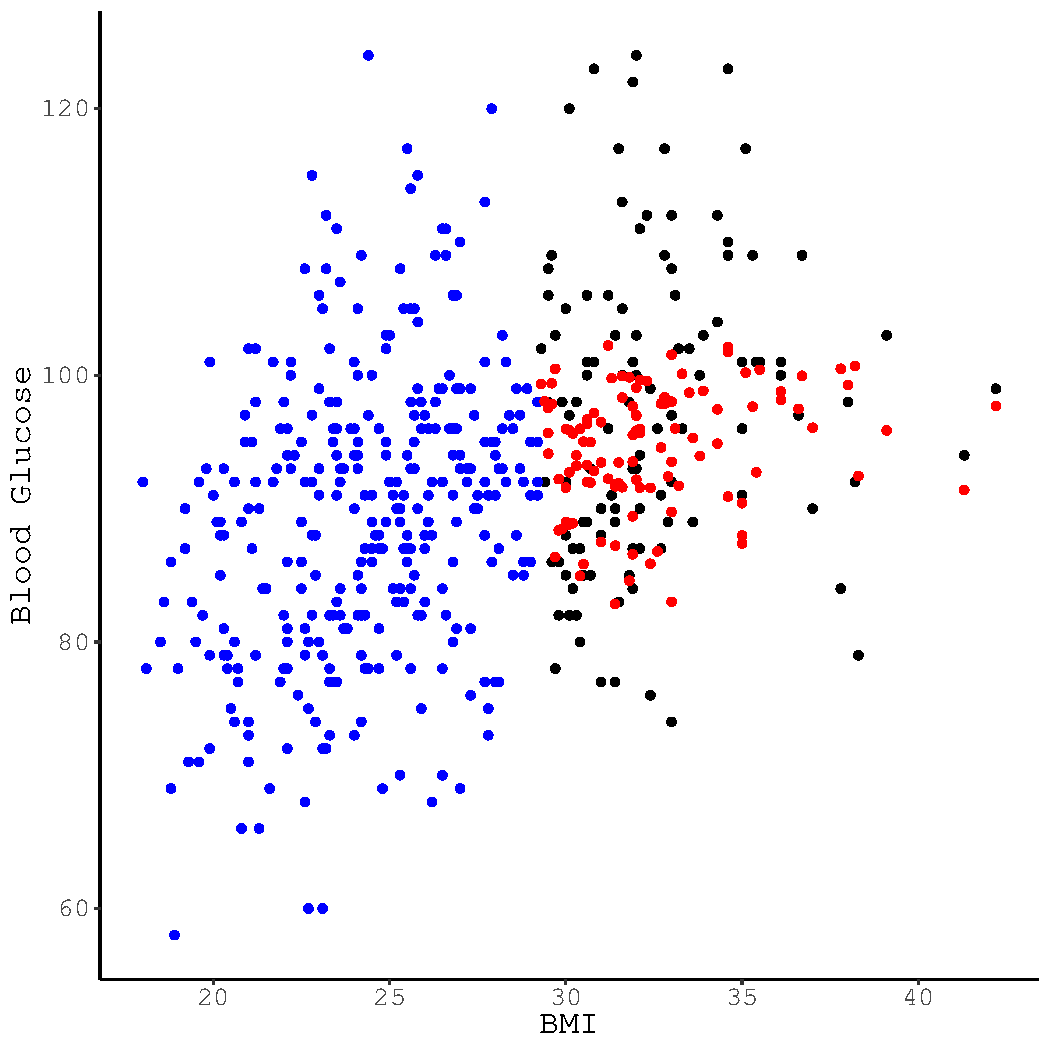
\includegraphics[width=\maxwidth]{figure/intro-unnamed-chunk-24-1} 

}


\end{knitrout}

\end{column}
\end{columns}

\end{frame}

%------------------------------------------------------------------------------%

\begin{frame}{Bad Methods (These almost never work)}
  
  \begin{center}
    \ovalbox{General Issues with Deletion-Based Methods}
  \end{center}
  
  \begin{itemize}
  \item Biased parameter estimates unless data are MCAR
  \item Generalizability issues
  \end{itemize}
  
  \va
  
  \begin{center}
    \ovalbox{General Issues with Simple Single Imputation Methods}
  \end{center}

  \begin{itemize}
  \item Biased parameter estimates even when data are MCAR
  \item Attenuates variability in any treated variables
  \end{itemize}
  
\end{frame}

%------------------------------------------------------------------------------%

\begin{frame}{Bad Methods (These almost never work)}
  
  Averaging Available Items (Person-Mean Imputation)
  \begin{itemize}
  \item Compute aggregate scores using only available values
    \begin{itemize}
    \item Missing data must be MCAR
    \item Each item must contributes equally to the aggregate score
    \end{itemize}
  \end{itemize}
  
  \vb
  
  Last Observation Carried Forward (LOCF)
  \begin{itemize}
  \item Replace post-dropout values with the most recent observed value
    \begin{itemize}
    \item Assume that dropouts would maintain their last known values
    \item Attenuates estimates of growth/development
    \end{itemize}
  \end{itemize}
  
\end{frame}

%------------------------------------------------------------------------------%

\begin{frame}{LOCF Viz}
  
\end{frame}

%------------------------------------------------------------------------------%

\begin{frame}{OK Methods (These work in some situations)}
  
  \begin{columns}
    \begin{column}{0.5\textwidth}
      
      Stochastic Regression Imputation
      \vc
      \begin{itemize}
      \item Fill $Y_{mis}$ with $\widehat{Y}_{mis}$ plus some random noise.
        \vc
        \begin{itemize}
        \item Produces unbiased parameter estimates and predictions
          \vc
        \item Computationally efficient
          \vc
        \item Attenuates standard errors
          \vc
        \item Makes CIs and prediction intervals too narrow
        \end{itemize}
      \end{itemize}
      
    \end{column}
    \begin{column}{0.5\textwidth}
      
\begin{knitrout}\footnotesize
\definecolor{shadecolor}{rgb}{0.878, 0.918, 0.933}\color{fgcolor}

{\centering 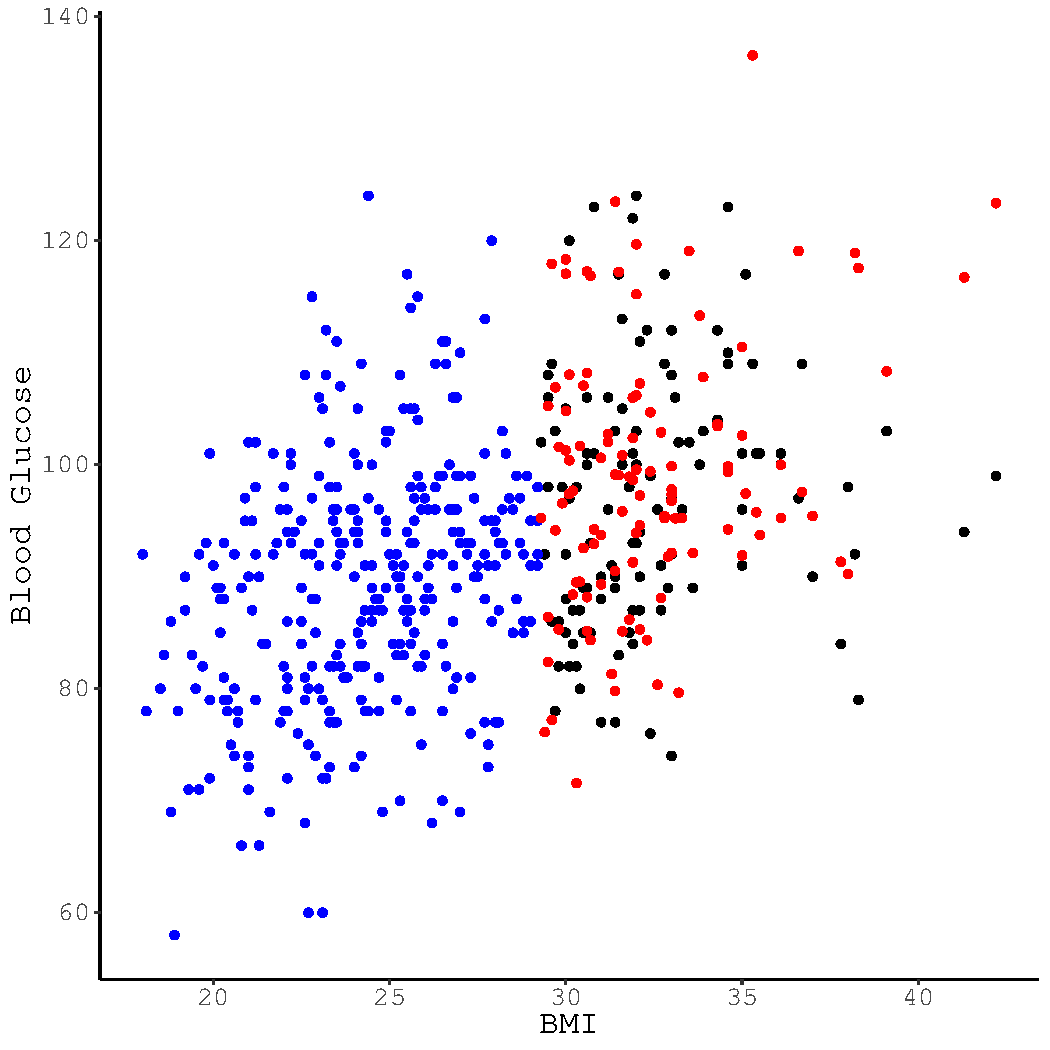
\includegraphics[width=\maxwidth]{figure/intro-unnamed-chunk-25-1} 

}


\end{knitrout}

\end{column}
\end{columns}

\end{frame}

\watermarkon %-----------------------------------------------------------------%

\begin{frame}{OK Methods (These work in some situations)}
  
  Nonresponse Weighting
  \vc
  \begin{itemize}
  \item Weight the observed cases to correct for nonresponse bias
    \vc
    \begin{itemize}
    \item Popular in survey research and official statistics
      \vc
    \item Only worth considering with \emph{Unit Nonresponse}
      \vc
    \item Doesn't make any sense with \emph{Item Nonresponse}
    \end{itemize}
  \end{itemize}
  
\end{frame}

%------------------------------------------------------------------------------%

\begin{frame}{Expectation Maximization}
  
\end{frame}

%------------------------------------------------------------------------------%

\begin{frame}{Good Methods (These almost always work)}
  
  Multiple Imputation (MI)
  \vc
  \begin{itemize}
  \item Replace the missing values with $M$ plausible estimates
    \vc
    \begin{itemize}
    \item Essentially, a repeated application of stochastic regression 
      imputation (with a particular type of regression model)
      \vc
    \item Produces unbiased parameter estimates and predictions
      \vc
    \item Produces ``correct'' standard errors, CIs, and prediction intervals
      \vc
    \item Very, very flexible
      \vc
    \item Computationally expensive
    \end{itemize}
  \end{itemize}
  
\end{frame}

\watermarkoff %----------------------------------------------------------------%

\begin{frame}[allowframebreaks, fragile]{Good Methods (These almost always 
    work)}

  What happens when we apply MI to our previous MAR example?
\begin{knitrout}\footnotesize
\definecolor{shadecolor}{rgb}{0.878, 0.918, 0.933}\color{fgcolor}\begin{kframe}
\begin{alltt}
\hlcom{## Estimate imputation model:}
\hlstd{miceOut1} \hlkwb{<-} \hlkwd{mice}\hlstd{(}\hlkwc{data}      \hlstd{=} \hlkwd{data.frame}\hlstd{(y3, x),}
                 \hlkwc{m}         \hlstd{=} \hlnum{100}\hlstd{,}
                 \hlkwc{maxit}     \hlstd{=} \hlnum{1}\hlstd{,}
                 \hlkwc{method}    \hlstd{=} \hlkwd{c}\hlstd{(}\hlstr{"norm"}\hlstd{,} \hlstr{""}\hlstd{),}
                 \hlkwc{printFlag} \hlstd{=} \hlnum{FALSE}\hlstd{)}

\hlcom{## Replace missing values with imputations:}
\hlstd{impList1} \hlkwb{<-} \hlkwd{list}\hlstd{()}
\hlkwa{for}\hlstd{(m} \hlkwa{in} \hlnum{1} \hlopt{:} \hlstd{miceOut1}\hlopt{$}\hlstd{m)}
    \hlstd{impList1[[m]]} \hlkwb{<-} \hlkwd{complete}\hlstd{(miceOut1, m)}
\end{alltt}
\end{kframe}
\end{knitrout}

\pagebreak

\begin{knitrout}\footnotesize
\definecolor{shadecolor}{rgb}{0.878, 0.918, 0.933}\color{fgcolor}\begin{kframe}
\begin{alltt}
\hlcom{## Estimate M correlations:}
\hlstd{corList} \hlkwb{<-}\hlkwd{lapply}\hlstd{(impList1,}
                 \hlkwc{FUN} \hlstd{=} \hlkwa{function}\hlstd{(}\hlkwc{impDat}\hlstd{)}
                     \hlkwd{cor}\hlstd{(impDat}\hlopt{$}\hlstd{x, impDat}\hlopt{$}\hlstd{y3)}
                 \hlstd{)}

\hlcom{## Pool estimates:}
\hlkwd{mean}\hlstd{(}\hlkwd{unlist}\hlstd{(corList))}
\end{alltt}
\begin{verbatim}
[1] 0.5108325
\end{verbatim}
\end{kframe}
\end{knitrout}

The MI-based parameter estimate looks good.
\begin{itemize}
\item MI produces unbiased estimates of the parameter when data are MAR.
\end{itemize}

\pagebreak

\begin{knitrout}\footnotesize
\definecolor{shadecolor}{rgb}{0.878, 0.918, 0.933}\color{fgcolor}

{\centering 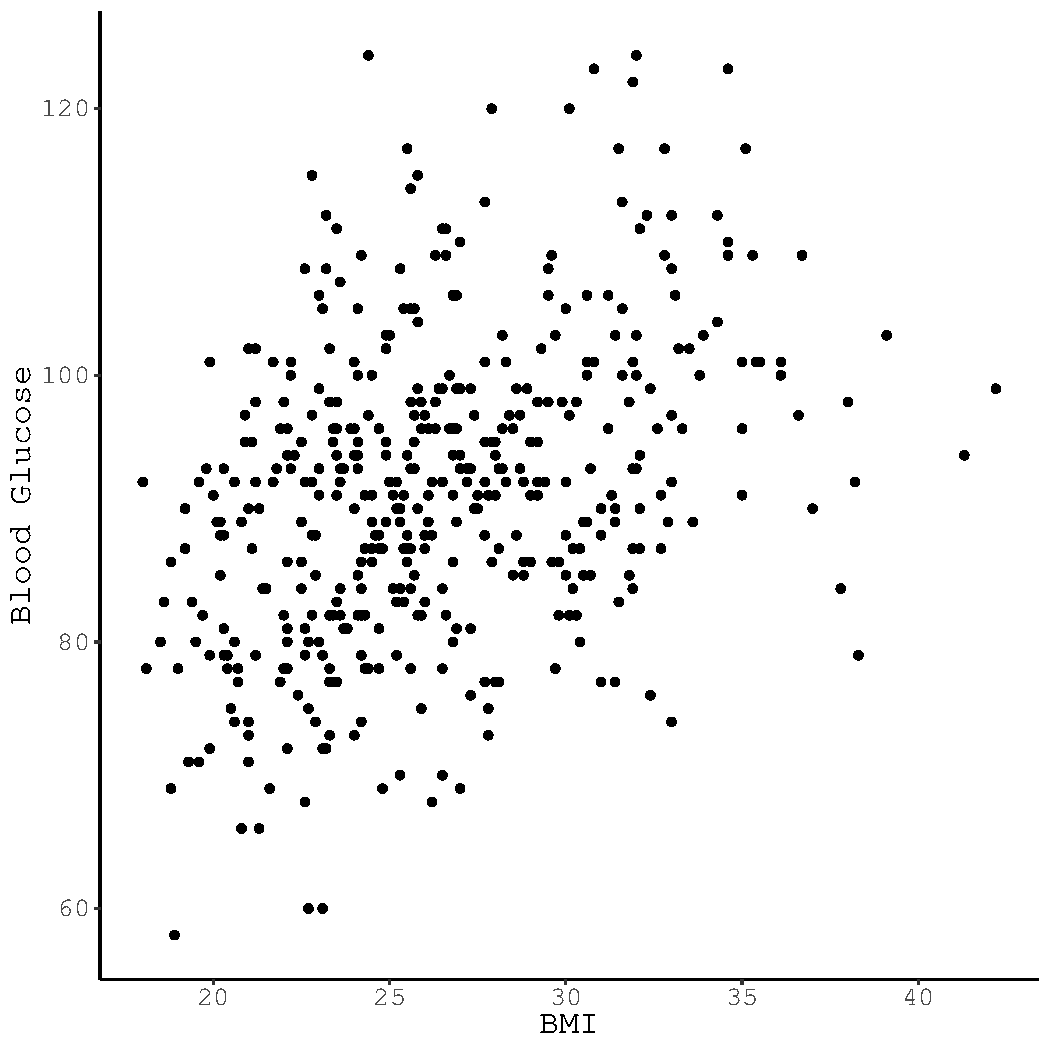
\includegraphics[width=0.65\linewidth]{figure/intro-unnamed-chunk-28-1} 

}


\end{knitrout}

\end{frame}

%------------------------------------------------------------------------------%

\begin{frame}[fragile]{Good Methods (These almost always work)}
  
  What about applying MI to our MNAR example?
\begin{knitrout}\footnotesize
\definecolor{shadecolor}{rgb}{0.878, 0.918, 0.933}\color{fgcolor}\begin{kframe}
\begin{alltt}
\hlcom{## Estimate imputation model:}
\hlstd{miceOut2} \hlkwb{<-} \hlkwd{mice}\hlstd{(}\hlkwc{data}      \hlstd{=} \hlkwd{data.frame}\hlstd{(y4, x),}
                 \hlkwc{m}         \hlstd{=} \hlnum{100}\hlstd{,}
                 \hlkwc{maxit}     \hlstd{=} \hlnum{1}\hlstd{,}
                 \hlkwc{method}    \hlstd{=} \hlkwd{c}\hlstd{(}\hlstr{"norm"}\hlstd{,} \hlstr{""}\hlstd{),}
                 \hlkwc{printFlag} \hlstd{=} \hlnum{FALSE}\hlstd{)}

\hlcom{## Replace missing values with imputations:}
\hlstd{impList2} \hlkwb{<-} \hlkwd{list}\hlstd{()}
\hlkwa{for}\hlstd{(m} \hlkwa{in} \hlnum{1} \hlopt{:} \hlstd{miceOut2}\hlopt{$}\hlstd{m)}
    \hlstd{impList2[[m]]} \hlkwb{<-} \hlkwd{complete}\hlstd{(miceOut2, m)}
\end{alltt}
\end{kframe}
\end{knitrout}

\end{frame}

%------------------------------------------------------------------------------%

\begin{frame}[allowframebreaks, fragile]{Good Methods (These \emph{almost} 
    always work)}

\begin{knitrout}\footnotesize
\definecolor{shadecolor}{rgb}{0.878, 0.918, 0.933}\color{fgcolor}\begin{kframe}
\begin{alltt}
\hlcom{## Estimate M correlations:}
\hlstd{corList2} \hlkwb{<-}\hlkwd{lapply}\hlstd{(impList2,}
                 \hlkwc{FUN} \hlstd{=} \hlkwa{function}\hlstd{(}\hlkwc{impDat}\hlstd{)}
                     \hlkwd{cor}\hlstd{(impDat}\hlopt{$}\hlstd{x, impDat}\hlopt{$}\hlstd{y4)}
                 \hlstd{)}

\hlcom{## Pool estimates:}
\hlkwd{mean}\hlstd{(}\hlkwd{unlist}\hlstd{(corList2))}
\end{alltt}
\begin{verbatim}
[1] 0.4089334
\end{verbatim}
\end{kframe}
\end{knitrout}

The MI-based parameter estimate is still biased.
\begin{itemize}
\item MI cannot correct bias in parameter estimates when data are MNAR.
\end{itemize}

\pagebreak

\begin{knitrout}\footnotesize
\definecolor{shadecolor}{rgb}{0.878, 0.918, 0.933}\color{fgcolor}

{\centering 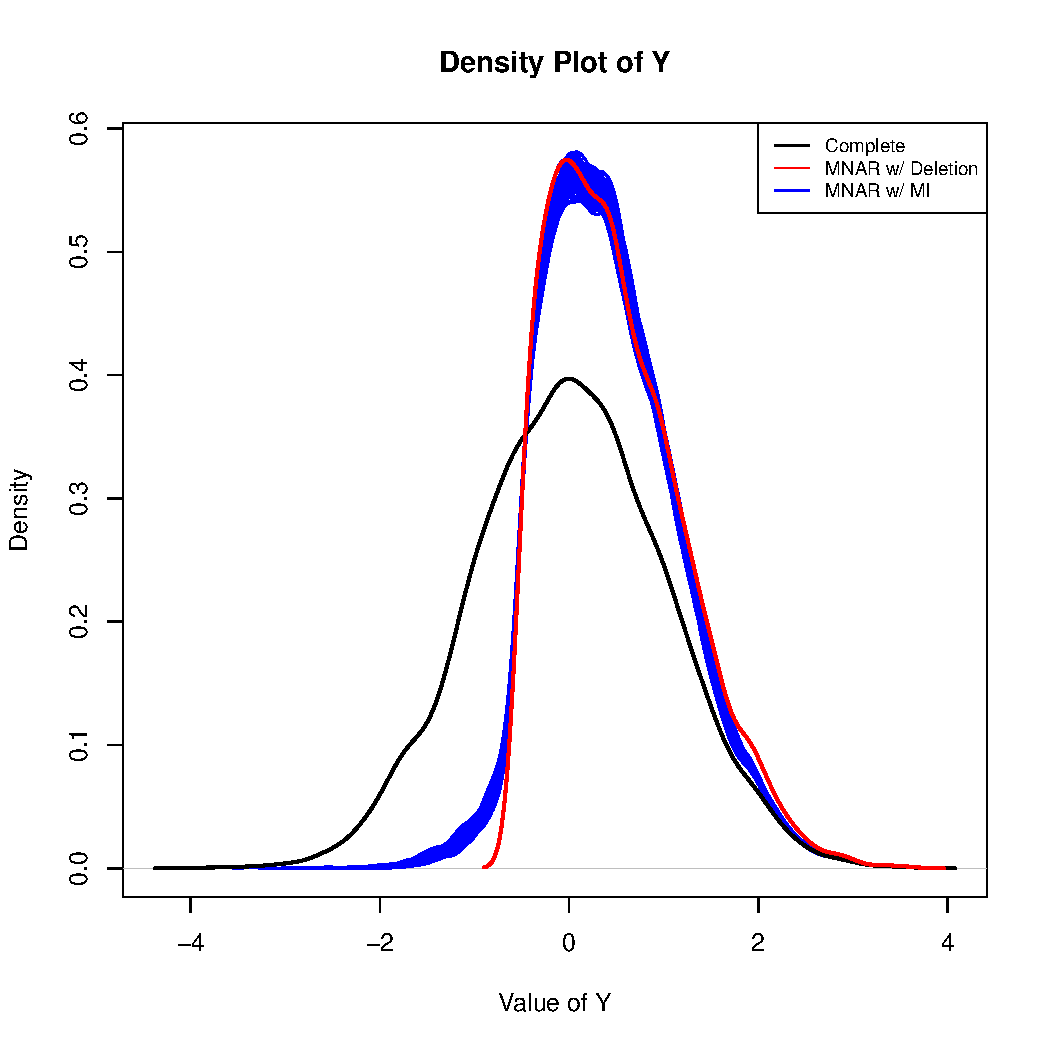
\includegraphics[width=0.65\linewidth]{figure/intro-unnamed-chunk-31-1} 

}


\end{knitrout}

\end{frame}

\watermarkon %-----------------------------------------------------------------%

\begin{frame}[allowframebreaks]{Good Methods (These almost always work)}

  Bayesian Modeling
  \vc
  \begin{itemize}
  \item Treat missing values as just another parameter to be estimated
    \vc
    \begin{itemize}
    \item Models can be directly estimated in the presence of missing data
      \begin{itemize}
      \item Essentially, runs MI behind-the-scenes during model estimation
      \end{itemize}
      \vc
    \item The predictors of nonresponse must be included in the model, somehow
      \vc
    \item Computationally expensive
    \end{itemize}
  \end{itemize}
  
  \pagebreak
  
  Full Information Maximum Likelihood (FIML)
  \vc
  \begin{itemize} 
  \item Adjust the objective function to only consider the observed parts of the 
    data
    \vc
    \begin{itemize}
    \item Models are directly estimated in the presence of missing data
      \vc
    \item The predictors of nonresponse must be included in the model, somehow
      \vc
    \item Unless you write your own optimization program, FIML is only available 
      for certain types of models
      \vc
    \item In linear regression models, FIML cannot treat missing data on 
      predictors (if the predictors are taken as fixed)
    \end{itemize}
  \end{itemize}
  
\end{frame}

%------------------------------------------------------------------------------%

\begin{frame}[allowframebreaks]{References}

  \bibliographystyle{apacite}
  \bibliography{../../../literature/bibtex/statMethRefs.bib}

\end{frame}

%------------------------------------------------------------------------------%

\end{document}
